% !TeX root = ../nxuthesis-example.tex

\chapter{图表、公式格式}

\section{图表格式}

图、表名中英文对照使用 \cs{bicaption} 命令来处理。

\begin{figure}
	\centering
	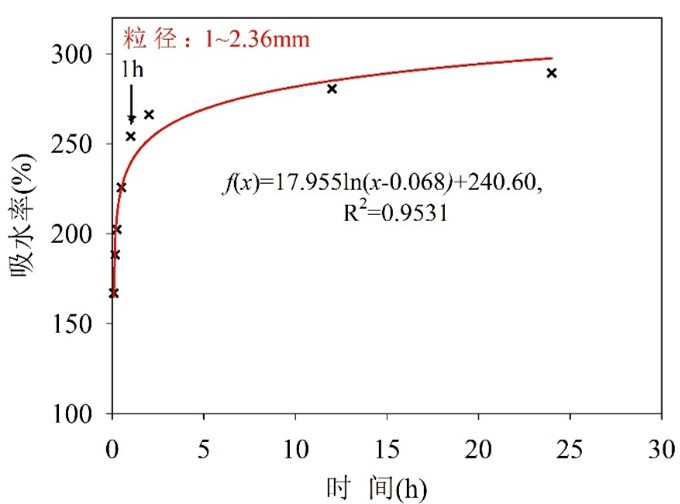
\includegraphics[]{figures/Figure 3-1.jpg}
	\bicaption{吸水率随时间的变化}{The change of water absorption rate with time}
	\label{Fig3-1}
	\begin{tablenotes}
		\item [a] 注:如有需要可对图片进行注释说明,可省略。
		\item [b] 资料来源:如需对图片来源进行说明,请参照此格式,可省略。 
	\end{tablenotes}
\end{figure}

\begin{table}
	\centering
	\bicaption{高频感应加热的基本参数}{XXXX}
	\begin{tabular}{cccc}
		\toprule
		\begin{tabular}[c]{@{}c@{}}感应频率\\(kHz)\end{tabular} & \begin{tabular}[c]{@{}c@{}}感应发生器功率\\(\%×80kW)\end{tabular} & \begin{tabular}[c]{@{}c@{}}工件移动速度\\(mm/min)\end{tabular} & \begin{tabular}[c]{@{}c@{}}感应圈与零件间隙\\(mm)\end{tabular} \\
		\midrule
		250 & 88 & 5900 & 1.65 \\
		250 & 88 & 5900 & 1.65 \\
		250 & 88 & 5900 & 1.65 \\
		250 & 88 & 5900 & 1.65 \\
		250 & 88 & 5900 & 1.65 \\
		250 & 88 & 5900 & 1.65 \\
		250 & 88 & 5900 & 1.65 \\
		250 & 88 & 5900 & 1.65 \\
		250 & 88 & 5900 & 1.65 \\
		250 & 88 & 5900 & 1.65 \\
		250 & 88 & 5900 & 1.65 \\
		\bottomrule
	\end{tabular}
	\begin{tablenotes}
		\item [a] 注:如有需要可对表格进行注释说明,可省略。
		\item [b] 资料来源:如需对表格来源进行说明,请参照此格式,可省略。 
	\end{tablenotes}
\end{table}

\section{公式格式}

\begin{equation}
	\sigma _{2C} = \frac{1+3.65\alpha}{(1+\alpha)^2} f'_C
\end{equation}

\section{插图示例}

图片通常在 \env{figure} 环境中使用 \cs{includegraphics} 插入,如图~\ref{fig:example} 的源代码。
建议矢量图片使用 PDF 格式,比如数据可视化的绘图;
照片应使用 JPG 格式;
其他的栅格图应使用无损的 PNG 格式。
注意,LaTeX 不支持 TIFF 格式;EPS 格式已经过时。

\begin{figure}
	\centering
	\includegraphics[width=0.5\linewidth]{example-image-a.pdf}
	\bicaption{示例图片标题}{XXX}
	\label{fig:example}
\end{figure}

若图或表中有附注,采用英文小写字母顺序编号,附注写在图或表的下方。
国外的期刊习惯将图表的标题和说明文字写成一段,需要改写为标题只含图表的名称,其他说明文字以注释方式写在图表下方,或者写在正文中。

如果一个图由两个或两个以上分图组成时,各分图分别以 (a)、(b)、(c)...... 作为图序,并须有分图题。
推荐使用 \pkg{subcaption} 宏包来处理, 比如图~\ref{fig:subfig-a} 和图~\ref{fig:subfig-b}。

\begin{figure}
	\centering
	\subcaptionbox{分图 A\label{fig:subfig-a}}
	{\includegraphics[width=0.35\linewidth]{example-image-a.pdf}}
	\subcaptionbox{分图 B\label{fig:subfig-b}}
	{\includegraphics[width=0.35\linewidth]{example-image-b.pdf}}
	\bicaption{多个分图的示例}{XXX}
	\label{fig:multi-image}
\end{figure}



\section{表格示例}

表应具有自明性。为使表格简洁易读,尽可能采用三线表,如表~\ref{tab:three-line}。
三条线可以使用 \pkg{booktabs} 宏包提供的命令生成。

\begin{table}
	\centering
	\bicaption{三线表示例}{XXX}
	\begin{tabular}{ll}
		\toprule
		文件名          & 描述                         \\
		\midrule
		thuthesis.dtx   & 模板的源文件,包括文档和注释 \\
		thuthesis.cls   & 模板文件                     \\
		thuthesis-*.bst & BibTeX 参考文献表样式文件    \\
		\bottomrule
	\end{tabular}
	\label{tab:three-line}
\end{table}

表格如果有附注,尤其是需要在表格中进行标注时,可以使用 \pkg{threeparttable} 宏包。
研究生要求使用英文小写字母 a、b、c……顺序编号,本科生使用圈码 ①、②、③……编号。

\begin{table}
	\centering
	\begin{threeparttable}[c]
		\bicaption{带附注的表格示例}{XXX}
		\label{tab:three-part-table}
		\begin{tabular}{ll}
			\toprule
			文件名                 & 描述                         \\
			\midrule
			thuthesis.dtx\tnote{a} & 模板的源文件,包括文档和注释 \\
			thuthesis.cls\tnote{b} & 模板文件                     \\
			thuthesis-*.bst        & BibTeX 参考文献表样式文件    \\
			\bottomrule
		\end{tabular}
		\begin{tablenotes}
			\item [a] 可以通过 xelatex 编译生成模板的使用说明文档;
			使用 xetex 编译 \file{thuthesis.ins} 时则会从 \file{.dtx} 中去除掉文档和注释,得到精简的 \file{.cls} 文件。
			\item [b] 更新模板时,一定要记得编译生成 \file{.cls} 文件,否则编译论文时载入的依然是旧版的模板。
		\end{tablenotes}
	\end{threeparttable}
\end{table}

如某个表需要转页接排,可以使用 \pkg{longtable} 宏包,需要在随后的各页上重复表的编号。
编号后跟表题(可省略)和“(续)”,置于表上方。续表均应重复表头。

\begin{longtable}{cccc}
	\bicaption{跨页长表格的表题}{XXX}
	\label{tab:longtable} \\
	\toprule
	表头 1 & 表头 2 & 表头 3 & 表头 4 \\
	\midrule
	\endfirsthead
	\caption*{续表~\thetable\quad 跨页长表格的表题} \\
	\toprule
	表头 1 & 表头 2 & 表头 3 & 表头 4 \\
	\midrule
	\endhead
	\bottomrule
	\endfoot
	Row 1  & & & \\
	Row 2  & & & \\
	Row 3  & & & \\
	Row 4  & & & \\
	Row 5  & & & \\
	Row 6  & & & \\
	Row 7  & & & \\
	Row 8  & & & \\
	Row 9  & & & \\
	Row 10 & & & \\
\end{longtable}



\section{算法示例}

算法环境可以使用 \pkg{algorithms} 或者 \pkg{algorithm2e} 宏包。

\renewcommand{\algorithmicrequire}{\textbf{输入:}\unskip}
\renewcommand{\algorithmicensure}{\textbf{输出:}\unskip}

\begin{algorithm}
	\caption{Calculate $y = x^n$}
	\label{alg1}
	\small
	\begin{algorithmic}
		\REQUIRE $n \geq 0$
		\ENSURE $y = x^n$
		
		\STATE $y \leftarrow 1$
		\STATE $X \leftarrow x$
		\STATE $N \leftarrow n$
		
		\WHILE{$N \neq 0$}
		\IF{$N$ is even}
		\STATE $X \leftarrow X \times X$
		\STATE $N \leftarrow N / 2$
		\ELSE[$N$ is odd]
		\STATE $y \leftarrow y \times X$
		\STATE $N \leftarrow N - 1$
		\ENDIF
		\ENDWHILE
	\end{algorithmic}
\end{algorithm}

\section{本章小结}

本章介绍了……